\documentclass[12pt]{article}

% Packages
\usepackage[utf8]{inputenc}
\usepackage{xeCJK}
\usepackage{ctex}
\usepackage{amsmath, amssymb}
\usepackage{graphicx}
\usepackage{hyperref}
\usepackage{geometry}
\usepackage{float}
\usepackage{cite}
\usepackage{subcaption}
\usepackage[linesnumbered,ruled,vlined]{algorithm2e}

% Page layout
\geometry{a4paper, margin=1in}

% Title and Author
\title{基于BSSMF矩阵分解的图像降噪方法}
\author{王伟钊}
\date{\today}

\begin{document}

\maketitle

\begin{abstract}

\end{abstract}

\newpage

\tableofcontents

\newpage

\section{绪论}
随着信息时代的快速发展,数字图像处理技术在各个领域得到了广泛的应用。然而,由于图像采集设备的限制,图像中常常会受到各种形式的噪声干扰。图像降噪是图像处理中的一个重要问题,其目的是去除图像中的噪声,使图像更加清晰,便于后续的图像分析和处理。图像降噪技术在医学图像处理、卫星图像处理、安防监控等领域有着广泛的应用。

\subsection{问题描述}
在数学上,图像降噪问题可以用如下数学表达式描述\cite{SVDWhiteNoise}:
\begin{equation}
    A(i,j)=A_{0}(i,j)+N(i,j)
\end{equation}
其中$A(i,j)$是观测到的图像,$A_{0}(i,j)$是原始图像,$N(i,j)$是噪声。噪声$N(i,j)$可以是各种形式的,图\ref{fig:noise_types}展示的是最常见的两种噪声:高斯白噪声和椒盐噪声。
\begin{figure}[H]
    \centering
    % 子图 (a)
    \begin{subfigure}[b]{0.45\textwidth}
        \centering
        
\includegraphics[width=\textwidth]{images/Gaussian_noise.png}
        \caption{高斯白噪声,$\mu$=0,$\sigma^2$=30}
    \end{subfigure}
    \hfill
    % 子图 (b)
    \begin{subfigure}[b]{0.45\textwidth}
        \centering
        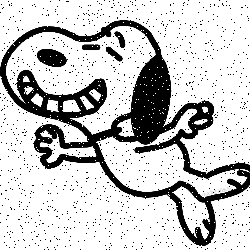
\includegraphics[width=\textwidth]{images/salt_pepper_noise.png}
        \caption{椒盐噪声}
    \end{subfigure}
    \caption{高斯白噪声和椒盐噪声}
    \label{fig:noise_types}
\end{figure}

本文主要关注高斯白噪声的降噪问题。高斯白噪声是一种均值为0,方差为$\sigma^2$的高斯分布,其概率密度函数为:

\begin{equation}
    f(x)=\frac{1}{\sqrt{2\pi}\sigma}e^{-\frac{(x - \mu)^{2}}{2\sigma^{2}}}
\end{equation}
其中$\mu$是均值,$\sigma$是标准差。由于大部分的白噪声均值为0,因此估计$\sigma$成为了图像降噪中的一个关键步骤,因为它直接影响降噪算法的性能。准确估计噪声水平可以帮助选择合适的降噪参数,从而在保留图像细节和去除噪声之间取得平衡。如果$\sigma$估计不准确,可能会导致过度平滑(损失细节)或降噪不足(残留噪声)\cite{Estimation_of_noise_variance}。为此,K. Rank等人\cite{MADestimate}使用绝对中位差(MAD)方法进行估计,Fabrizio Russo等人\cite{AWGN}在2003年提出了一种基于新型滤波器对标准差$\sigma$进行估计的方法。Liu等人在2013年提出了基于SVD的方法\cite{SVDWhiteNoise}进行估计。有了准确的噪声估计,我们就可以选择合适的降噪算法对图像进行降噪。

\subsection{国内外图像降噪算法研究现状}
随着人工智能的时代到来,图像降噪算法也经历了从传统方法到深度学习方法的转变。传统的图像降噪方法主要依赖于图像的先验知识和统计特性,而深度学习方法则通过大量的数据训练来自动学习图像的特征,从而实现更好的降噪效果。

\subsubsection{基于传统滤波器的方法}
传统的图像降噪方法主要包括均值滤波、中值滤波和高斯滤波等。这些方法通过对图像进行平滑处理来去除噪声,均值滤波是一种简单的线性滤波方法,通过对图像中每个像素点周围的像素值进行平均来平滑图像。中值滤波是一种非线性滤波方法,通过对图像中每个像素点周围的像素值进行排序,然后取中间值来平滑图像。高斯滤波是一种加权平均滤波方法,通过对图像中每个像素点周围的像素值进行加权平均来平滑图像。赵等人在2011年提出了一种能加速中值滤波算法计算的方法,使得中值滤波的效果更好以及计算更快\cite{中值滤波}。这些传统方法的底层逻辑十分简单,容易实现,但在处理复杂噪声时效果较差,且容易导致图像细节的损失,边缘模糊。

\subsubsection{基于小波变换的方法}
小波变换是一种时频分析方法,可以有效地提取图像的多尺度特征。基于小波变换的图像降噪方法通过对图像进行小波变换,将图像分解为不同频率的子带,然后对高频子带进行阈值处理,最后再进行小波逆变换来重构图像。徐等人在2022年提出了一种改进的小波软阈值函数\cite{小波变换},使得小波变换的去噪效果明显提升,这种方法可以有效地去除高频噪声,同时保留低频信息。但是,小波变换方法在处理图像边缘和细节时可能会出现伪影现象,导致图像质量下降。同时阈值函数的超参数的确定也会影响图片降噪效果。

\subsubsection{基于深度学习的方法}
近年来,深度学习在图像处理领域取得了显著的进展。基于深度学习的图像降噪方法主要包括卷积神经网络(CNN)和生成对抗网络(GAN)等\cite{深度学习去噪},以及基于注意力机制的图像降噪方法\cite{注意力机制}。这些方法通过训练深度神经网络来学习图像的特征,从而实现图像降噪。与传统方法相比,基于深度学习的方法在处理复杂噪声和保留图像细节方面表现更好。但是,这些方法通常需要大量的训练数据和计算资源,且对网络结构和参数的选择较为敏感。目前为止,仍然没有理论上的证明来说明深度学习方法的收敛性和稳定性。

\subsection{本文的研究内容}
本文主要研究基于有界单纯形矩阵分解(Bounded Simplex Structured Matrix Factorization, BSSMF)矩阵分解的图像降噪方法。BSSMF算法是一种结合了非负矩阵分解(NMF)和结构化矩阵分解(SSMF)的矩阵分解算法。本文将BSSMF算法应用于图像降噪中,提出了一种新的图像降噪方法,并通过实验验证了其有效性。
本文的主要贡献包括:
\begin{itemize}
    \item 提出了一种基于BSSMF矩阵分解的图像降噪方法,通过对图像进行矩阵分解来去除噪声。
    \item 设计了一种新的BSSMF算法,通过引入特定的边界条件和概率单纯形约束来提高算法的性能。
    \item 通过实验验证了所提出的方法在不同噪声水平下的有效性,并与传统方法进行了对比分析。
\end{itemize}

\newpage

\section{相关工作}
矩阵分解问题在数学上可以表示为:
\begin{equation}
    X \approx WH
    \label{eq:matrix_decomposition}
\end{equation}
其中$X\in \mathbb{R}^{m \times n}$是原始矩阵,$W \in \mathbb{R}^{m \times r}$和$H \in \mathbb{R}^{r \times n}$是目标矩阵。矩阵分解要求$r\ll min(m, n)$\cite{NMFIdentifiability},从而实现对原始矩阵的有效压缩和重构。后人们在此基础上加上了不同的约束条件,提出了多种矩阵分解算法,如非负矩阵分解(NMF)\cite{NMF}、稀疏矩阵分解(SMF)\cite{SMF}、结构化矩阵分解(SSMF)\cite{SSMF2}\cite{SSMF1}等。
\subsection{BSSMF算法}
BSSMF(Bounded Sparse and Structured Matrix Factorization)\cite{BSSMF}是一种矩阵分解算法,旨在从给定的矩阵中提取出潜在的结构化信息。BSSMF算法结合了NMF算法和SSMF算法,通过引入稀疏性约束和结构化约束来实现对矩阵的有效分解。该算法的主要思想是将\eqref{eq:matrix_decomposition}中的$W$和$H$矩阵进行约束,使得它们在分解过程中$W$满足边界条件\eqref{Bounded},

\begin{equation}
    W(i,j) \in [a, b] \quad \forall i,j
    \label{Bounded}
\end{equation}
而$H$矩阵满足单纯形约束\eqref{Simplex}:
\begin{equation}
    \Delta^r = \left\{ H \in \mathbb{R}^{r \times n} : H_{ij} \geq 0, \sum_{i=1}^{r} H_{ij} = 1, j=1,2,\ldots,n \right\}
    \label{Simplex}
\end{equation}

BSSMF算法的目标是最小化以下目标函数:
\begin{equation}
    f = \min_{W,H} \frac{1}{2}\left\lVert X - WH \right\rVert_F^2 
    \label{Loss}
\end{equation}
其中$\lambda_1$和$\lambda_2$是正则化参数,$\left\lVert \cdot \right\rVert_F$表示Frobenius范数,$\left\lVert \cdot \right\rVert_2$表示L2范数。BSSMF算法通过迭代优化$W$和$H$矩阵,使得目标函数达到最小值。

迭代过程中,BSSMF算法使用了梯度下降法,分别对目标函数\eqref{Loss}的$W$和$H$进行求梯度,得到以下更新公式:

\begin{equation}
    \nabla f_W = -\left( X - WH \right)H^T
    \label{Gradient_W}
\end{equation}

\begin{equation}
    \nabla f_H = -W^T\left( X - WH \right)
    \label{Gradient_H}
\end{equation}
BSSMF算法通过迭代更新$W$和$H$,使得目标函数逐渐收敛到最小值。


以下是BSSMF算法\ref{algo}的计算过程:

\begin{algorithm}[H]
    \SetKwData{Left}{left}\SetKwData{This}{this}\SetKwData{Up}{up}
    \SetKwFunction{Union}{Union}\SetKwFunction{FindCompress}{FindCompress}
    \SetKwInOut{Input}{input}\SetKwInOut{Output}{output}
  
    \Input{ matrix $X \in \mathbb{R}^{m \times n}$, bounds $a\leqslant b \in \mathbb{R}$, initial factors $W \in \mathbb{R}^{m \times r}$ s.t.
    
    $W(:,k)\in [a,b]$ for all $k$ and simplex structured $H \in \mathbb{R}^{r \times n}_{+}$ , weights $M \in [0, 1]^{m \times n}$}
    \Output{$W$ and $H$}

    { $\alpha_1 = 1$, $\alpha_2 = 1$, $W_{old} = W$, $H_{old} = H$, $L^{prev}_W = L_W = \left\lVert HH^T\right\rVert_2, L^{prev}_H = L_H = \left\lVert WW^T\right\rVert_2$ }

    \Repeat{$some\ stopping\ criteria\ is\ satisfied$}{
        \While{$stopping\ criteria\ not\ satisfied$}{$
            \alpha_0 = \alpha_1 , \alpha_1 = (1+\sqrt{1+4\alpha_1^2})/2$

            $\beta_W = min\left[ (\alpha_0 - 1)/\alpha_1, 0.9999\sqrt{L^{prev}_W/L_W} \right]$

            $\overline{W} \leftarrow W + \beta_W (W - W_{old})$

            $W_{old} \leftarrow W$
            
            $W \leftarrow \left[ \overline{W} + \frac{M \odot (X - \overline{W}H)H^T}{L_W} \right]^a_b$

            $L^{prev}_W = L_W$
            }
        $L_H \leftarrow \left\lVert W^TW\right\rVert_2$
        
        \While{$stopping\ criteria\ not\ satisfied$}{$
            \alpha_0 = \alpha_2 , \alpha_2 = (1+\sqrt{1+4\alpha_2^2})/2$

            $\beta_H = min\left[ (\alpha_0 - 1)/\alpha_2, 0.9999\sqrt{L^{prev}_H/L_H} \right]$

            $\overline{H} \leftarrow H + \beta_H (H - H_{old})$

            $H_{old} \leftarrow H$
            
            $H \leftarrow \left[ \overline{H} + \frac{W^T(M \odot (X - W\overline{H}))}{L_H} \right]_{\Delta^r}$

            $L^{prev}_H = L_H$
            }
        $L_W = \left\lVert H^TH\right\rVert_2$
    }
    
    \caption{BSSMF算法}
    \label{algo}
    \small 注*:$L_W $和$L_H$分别表示$W$和$H$的L2范数,可以有效控制算法速度,且能在有部分数据为缺失的情况下进行收敛\cite{Lip}。
    
  \end{algorithm}\DecMargin{1em}

在原始的BSSMF算法中,可以用$n$张具有相同特征的图片转为$n$个一维向量,每张图片像素点的个数即为$m$,然后将n个向量拼接为$m\times n$的输入矩阵$X$,算法运行后输入矩阵$X$的列可以近似表示为$W$矩阵中列的线性组合,即:
\begin{equation}
    X(:,j) \approx \sum_{i=1}^{r} W(:,i)H(i,j)
\end{equation}
由于$H$矩阵满足单纯形约束,因此$H(i,j)$的值在$[0,1]$之间且加和为1,这更直观地说明了$X$的组成成分。在算法中对$W$进行[0,255]的约束,可以使分解后的$W$直接对应一张图片,更直观的解释了算法的可解释性。因此BSSMF算法通过对输入矩阵进行分解,可以提取出潜在的特征信息,从而实现对数据的降维和特征选择。图\ref{fig:BSSMF1}展示了BSSMF算法和NMF算法在MNIST数据集上的分解结果。可以看出,BSSMF算法能够更清晰地提取出数字间共同的特征,而NMF算法则存在一定的模糊性。图\ref{fig:BSSMF2}展示了数字8的BSSMF分解结果,以及最后的组合方式。可以看出,BSSMF算法能够有效地提取出数字8的特征信息,并且通过对特征进行组合,可以重构出原始图像\cite{BSSMF}。
\begin{figure}[H]
    \centering
    % 子图 (a)
    \begin{subfigure}[b]{0.45\textwidth}
        \centering
        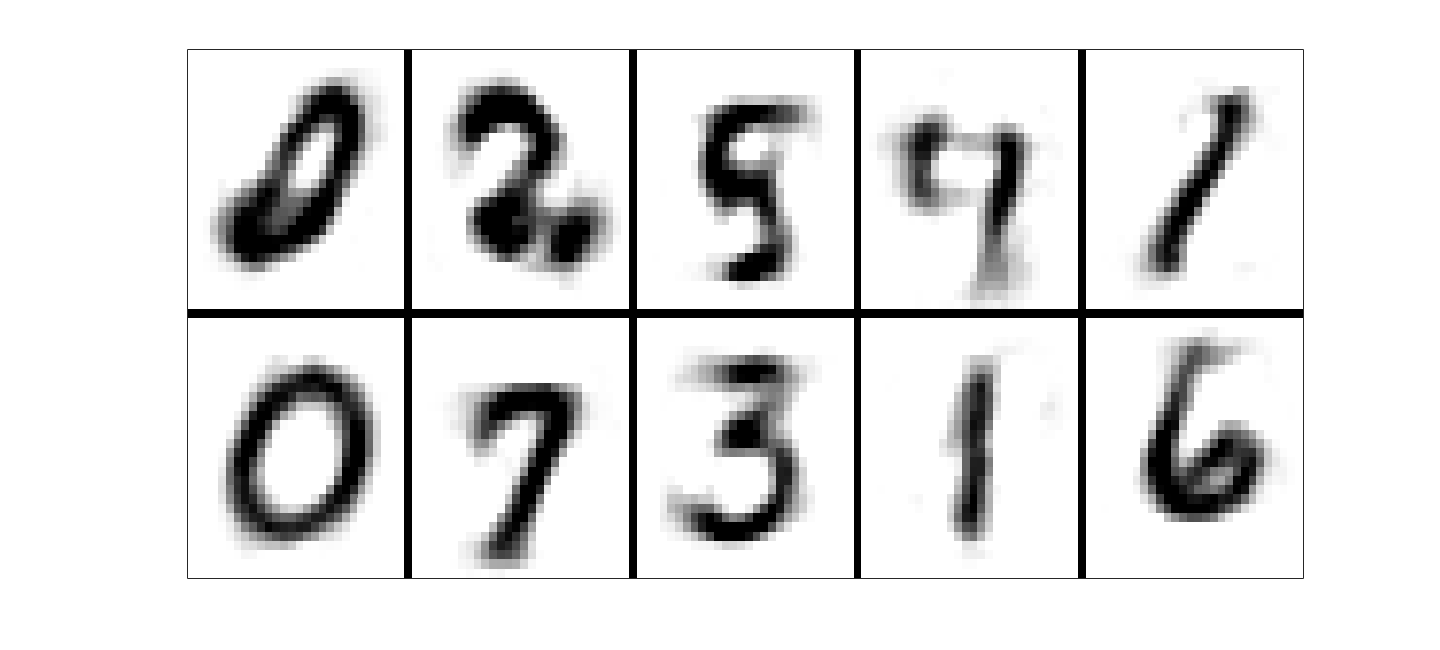
\includegraphics[width=\textwidth]{images/BSSMF_MNIST.png}
        \caption{BSSMF}
    \end{subfigure}
    \hfill
    % 子图 (b)
    \begin{subfigure}[b]{0.45\textwidth}
        \centering
        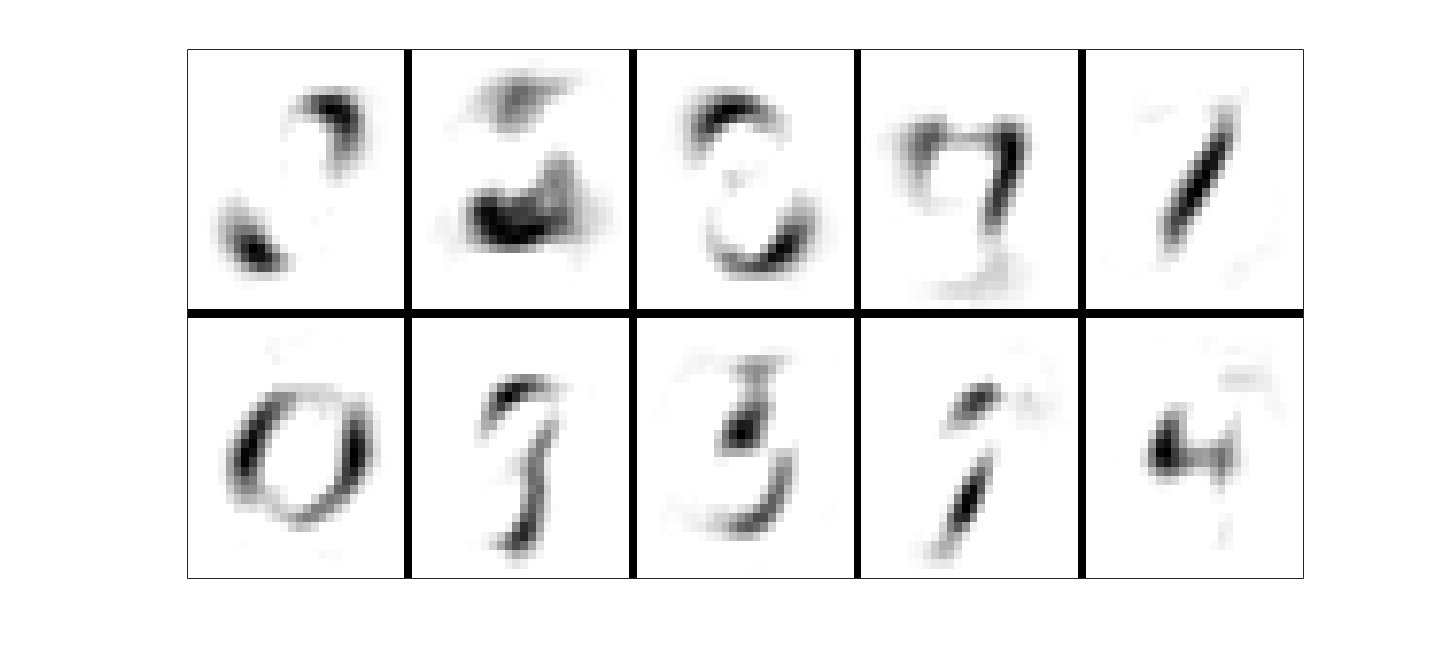
\includegraphics[width=\textwidth]{images/NMF_MNIST.png}
        \caption{NMF}
    \end{subfigure}
    \caption{BSSMF和NMF基于500张数字图像分解到$r=10$的对比}
    \caption*{\raggedright \small 注*:每一张图片代表$W$矩阵中的一列经过reshape函数处理后的结果}
    \label{fig:BSSMF1}
\end{figure}

\begin{figure}[H]
    \centering
    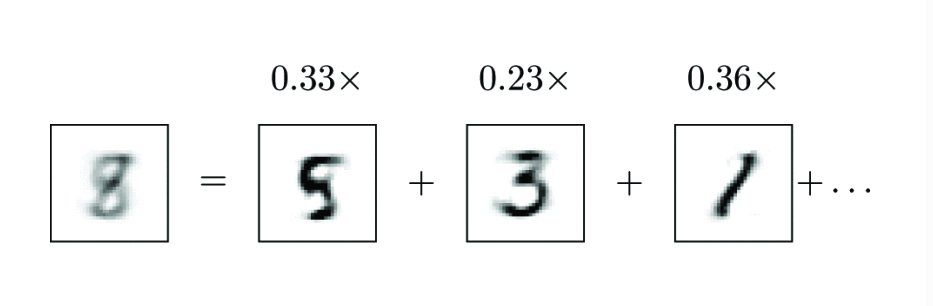
\includegraphics[width=\textwidth]{images/deconposition.png}
    \caption{数字8的BSSMF分解}
    \label{fig:BSSMF2}
\end{figure}

\subsection{设定特定边界条件的BSSMF算法}

有了对BSSMF算法的初步了解后,我们可以对其进行改进。BSSMF算法的一个缺点是分解后的$W$矩阵所有的列向量都在$[a,b]$的范围内,这使得分解后的$W$矩阵的每一列都具有相同的边界条件,这在某些情况下可能不符合实际需求。例如,在图像降噪中,我们更希望分解后的$W$矩阵在前几列或第一列保留图像的最关键信息,而后面的列则只包含噪声信息$N$。为了解决这个问题,我们可以对BSSMF算法进行改进,设定特定的边界条件,使得分解后的$W$矩阵的每一列都具有不同的边界条件。我们可以将$W$矩阵的前$r_1$列设定为$[a_1,b_1]$,后$r_2$列设定为$[a_2,b_2]$,其中$r_1+r_2=r$。这样,我们就可以在分解后的$W$矩阵中保留图像的最关键信息,同时去除噪声信息。如下图\ref{fig:matrix_decomposition}所示,假设$W$矩阵的$W_{i1}$设定为$[0,255]$,$W_{i2}$和$W_{i3}$设定为$[0,30]$。这样,我们在分解后的$W$矩阵中便能将图像的最关键信息保存在第1列,而噪声等其他信息保存在第2第3列。
\begin{figure}[H]
    \centering
    \begin{equation*}
        \begin{bmatrix}
            x_{11} & x_{12} & x_{13} & x_{14} \\
            x_{21} & x_{22} & x_{23} & x_{24} \\
            x_{31} & x_{32} & x_{33} & x_{34} \\
            x_{41} & x_{42} & x_{43} & x_{44} \\
        \end{bmatrix}
        =
        \begin{bmatrix}
            w_{11} & w_{12} & w_{13}\\
            w_{21} & w_{22} & w_{23} \\
            w_{31} & w_{32} & w_{33} \\
            w_{41} & w_{42} & w_{43}

        \end{bmatrix}
        \cdot
        \begin{bmatrix}
            h_{11} & h_{12} & h_{13} & h_{14} \\
            h_{21} & h_{22} & h_{23} & h_{24} \\
            h_{31} & h_{32} & h_{33} & h_{34} \\
        \end{bmatrix}
    \end{equation*}
    \caption{矩阵分解}
    \label{fig:matrix_decomposition}
\end{figure}

除去对分解矩阵$W$第一列的约束为$[0,255]$外,我们应如何确定其他列的边界条件呢?基于高斯白噪声的概率学特性,可以找到绝大部分的噪声幅值所存在的范围。我们可以通过噪声的Z分位数来确定其他列的边界条件。

Z分位数是一种用于描述数据分布的统计量,可以用于评估数据的集中趋势和离散程度。Z分位数的计算可用以下公式\ref{eq:Z}表示:
\begin{equation}
    Z = \frac{X - \mu}{\sigma}
    \label{eq:Z}
\end{equation}
其中$X$是数据值,$\mu$是均值,$\sigma$是标准差。Z分位数所对应的概率值可以通过查找Z分位数表\ref{tab:z_table_detailed}计算获得。其内容为:在标准正态分布下($\mu = 0 , \sigma = 1 $),随机变量$X$在$P(X \leq z)$的概率。该表列出了不同分位数对应的Z值,可以用于快速查找和计算。

普通加性高斯白噪声的均值为$\mu$,标准差为$\sigma$,我们可以通过查找Z分位数表\ref{tab:z_table_detailed}来确定噪声的幅值范围。假设我们希望分解能够包含95\%的噪声,我们可以查找Z分位数表中对应于97.5\%的Z值为1.96。根据公式\ref{eq:Z},我们可以计算出噪声幅值范围为:
\begin{equation}
    X \in [\mu - 1.96\sigma, \mu + 1.96\sigma] = [\mu -1.96\sigma,\mu + 1.96\sigma]
\end{equation}
因此,我们可以将$W$矩阵的后几列的边界条件设定为$[\mu -1.96\sigma,\mu + 1.96\sigma]$。

举一个例子,我们有一个高斯白噪声的图像,其均值为10,标准差为20。我们可以通过查找Z分位数表来确定噪声的幅值范围。我们希望分解能够包含99\%的噪声,我们可以查找Z分位数表中对应于99\%的Z值为2.576。根据公式\ref{eq:Z},我们可以计算出噪声幅值范围为:
\begin{equation}
    X \in [10 - 2.576 \times 20, 10 + 2.576 \times 20] = [-41.52, 61.52]
\end{equation}
因此,我们可以将$W$矩阵的后几列的边界条件设定为$[-41.52, 61.52]$。这样,我们就可以在分解后的$W$矩阵中保留图像的最关键信息,同时分离噪声信息。

\subsection{对概率单纯形的改进}


\subsection{基于BSSMF的图像降噪算法}

\newpage
\section{实验结果与分析}
\subsection{实验设计}

\newpage
\section{结论}

\bibliographystyle{plain}
\bibliography{ref}

\appendix
\section*{\centering \Huge 附录}

\section{标准正态分布的Z分位数表}
\begin{table}[H]
    \centering
        \caption{\small 标准正态分布Z分位数表}
        \label{tab:z_table_detailed}
        \begin{tabular}{|c|c|c|c|c|c|c|c|c|c|c|}
            \hline
            Z值 & 0.00 & 0.01 & 0.02 & 0.03 & 0.04 & 0.05 & 0.06 & 0.07 & 0.08 & 0.09 \\ \hline
            0.0 & 0.5000 & 0.5040 & 0.5080 & 0.5120 & 0.5160 & 0.5199 & 0.5239 & 0.5279 & 0.5319 & 0.5359 \\ \hline
            0.1 & 0.5398 & 0.5438 & 0.5478 & 0.5517 & 0.5557 & 0.5596 & 0.5636 & 0.5675 & 0.5714 & 0.5753 \\ \hline
            0.2 & 0.5793 & 0.5832 & 0.5871 & 0.5910 & 0.5948 & 0.5987 & 0.6026 & 0.6064 & 0.6103 & 0.6141 \\ \hline
            0.3 & 0.6179 & 0.6217 & 0.6255 & 0.6293 & 0.6331 & 0.6368 & 0.6406 & 0.6443 & 0.6480 & 0.6517 \\ \hline
            0.4 & 0.6554 & 0.6591 & 0.6628 & 0.6664 & 0.6700 & 0.6736 & 0.6772 & 0.6808 & 0.6844 & 0.6879 \\ \hline
            0.5 & 0.6915 & 0.6950 & 0.6985 & 0.7019 & 0.7054 & 0.7088 & 0.7123 & 0.7157 & 0.7190 & 0.7224 \\ \hline
            0.6 & 0.7257 & 0.7291 & 0.7324 & 0.7357 & 0.7389 & 0.7422 & 0.7454 & 0.7486 & 0.7517 & 0.7549 \\ \hline
            0.7 & 0.7580 & 0.7611 & 0.7642 & 0.7673 & 0.7704 & 0.7734 & 0.7764 & 0.7794 & 0.7823 & 0.7852 \\ \hline
            0.8 & 0.7881 & 0.7910 & 0.7939 & 0.7967 & 0.7995 & 0.8023 & 0.8051 & 0.8078 & 0.8106 & 0.8133 \\ \hline
            0.9 & 0.8159 & 0.8186 & 0.8212 & 0.8238 & 0.8264 & 0.8289 & 0.8315 & 0.8340 & 0.8365 & 0.8389 \\ \hline
            1.0 & 0.8413 & 0.8438 & 0.8461 & 0.8485 & 0.8508 & 0.8531 & 0.8554 & 0.8577 & 0.8599 & 0.8621 \\ \hline
            1.1 & 0.8643 & 0.8665 & 0.8686 & 0.8708 & 0.8729 & 0.8749 & 0.8770 & 0.8790 & 0.8810 & 0.8830 \\ \hline
            1.2 & 0.8849 & 0.8869 & 0.8888 & 0.8907 & 0.8925 & 0.8944 & 0.8962 & 0.8980 & 0.8997 & 0.9015 \\ \hline
            1.3 & 0.9032 & 0.9049 & 0.9066 & 0.9082 & 0.9099 & 0.9115 & 0.9131 & 0.9147 & 0.9162 & 0.9177 \\ \hline
            1.4 & 0.9192 & 0.9207 & 0.9222 & 0.9236 & 0.9251 & 0.9265 & 0.9279 & 0.9292 & 0.9306 & 0.9319 \\ \hline
            1.5 & 0.9332 & 0.9345 & 0.9357 & 0.9370 & 0.9382 & 0.9394 & 0.9406 & 0.9418 & 0.9429 & 0.9441 \\ \hline
            1.6 & 0.9452 & 0.9463 & 0.9474 & 0.9484 & 0.9495 & 0.9505 & 0.9515 & 0.9525 & 0.9535 & 0.9545 \\ \hline
            1.7 & 0.9554 & 0.9564 & 0.9573 & 0.9582 & 0.9591 & 0.9599 & 0.9608 & 0.9616 & 0.9625 & 0.9633 \\ \hline
            1.8 & 0.9641 & 0.9649 & 0.9656 & 0.9664 & 0.9671 & 0.9678 & 0.9686 & 0.9693 & 0.9699 & 0.9706 \\ \hline
            1.9 & 0.9713 & 0.9719 & 0.9726 & 0.9732 & 0.9738 & 0.9744 & 0.9750 & 0.9756 & 0.9761 & 0.9767 \\ \hline
            2.0 & 0.9772 & 0.9778 & 0.9783 & 0.9788 & 0.9793 & 0.9798 & 0.9803 & 0.9808 & 0.9812 & 0.9817 \\ \hline
        \end{tabular}
        \caption*{\raggedright \small 注:该表展示了标准正态分布的Z分位数,Z值表示标准正态分布曲线下的累积概率。}
\end{table}

\end{document}